% !TeX spellcheck = en_US
\section{Problem 3}

LVQ (Learning Vector Quantization) is a type of artificial neural network algorithm used for supervised learning. It belongs to the category of competitive learning algorithms and is particularly effective for classification tasks.

\begin{figure}[htpb]
	\centering
	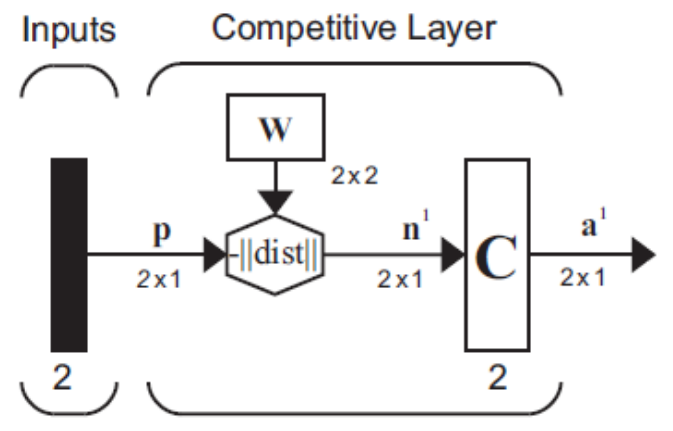
\includegraphics[width=0.4\linewidth]{../Problem 3/prob3_lvq_nn.png}
	\caption{Given neural network.}
\end{figure}

The following $-||w_i - p||$ applies to every $n^1_i$. Also, we can also state that $a^1 = compet\left(n^1\right)$, where $compet$ is competitive learning layer.

During training, the distance between $a$ and $w$ is calculated using $dist = norm\left(p-w_{1,2}\right)$ and judging by whose norm is grater, the winning neutron gets updated.